\documentclass[11pt,a4paper]{article}

\usepackage[utf8]{inputenc}
\usepackage[T1]{fontenc}
\usepackage{amsmath,amssymb,amsfonts}
\usepackage{graphicx}
\usepackage{hyperref}
\usepackage{booktabs}
\usepackage{enumitem}
\usepackage[margin=2.5cm]{geometry}
\usepackage{parskip}
\usepackage{xcolor}
\usepackage{pifont}
\usepackage[margin=0.5cm]{caption}
\usepackage{changepage}
\usepackage{array}
\usepackage{arydshln}
\usepackage{rotating}

\newcommand{\cmark}{{\color{green!70!black}\ding{51}}}
\newcommand{\xmark}{{\color{red}\ding{55}}}
\newcommand{\rothead}[1]{\rotatebox[origin=c]{60}{\smash{\textbf{#1}}}}

\title{Transformer Toy Model Sequence Memorisation}
\author{}
\date{}

\begin{document}
\maketitle

\section{Why sequence memorisation}
We expect that a lot of the information stored in the weights of a transformer is memorised facts, rather than general circuits. 

\section{The training data}
The training data are seqences of three token, one two input tokens and one output token. Given an input of tow tokens, the network is trained to predict the next token (i.e. the output token). 

Hyper parameters for the data generation:
\begin{itemize}
    \item input token vocabulary size
    \item output token vocabulary size
\end{itemize}

In our experiments, the input token vocabulary size is always twise the size as the output token vocabulary size.\footnote{We started out the experiments, having them the same size, but the network learned all the facts to easaly, so we dubbled the input vocabulary size in order to have more possible facts.}

\subsection{Generating the training data}

The code for generating the training data is not very long, and is quoted below if you prefeer to read code. 

The inputs are 
\begin{itemize}
    \item \verb|n_facts| -- Number of facts.
    \item \verb|input_len| -- Number of input tokens. \emph{This value is aways 2.}
    \item \verb|input_vocal_size|
    \item \verb|output_vocab_size|
    \item \verb|seed| -- Random seed. \emph{This value is always 42.}\footnote{We used a fixed random seed to avoid some runs getting lucky and getting easier fracts, and to specifically have the same facts for trained networks and hand-coded networks. However this last aim failed becasuse torch random functions give diffrent results diffrent when run on CPU vs GPU, even with the seed is the same. However, this probably isn't significant a significant concern.}
\end{itemize}

The code first generates a list of every possible input combination. Then this list is shuffled, and the first \verb|n_fact| pairs from the shuffled list are used as the inputs for the \verb|n_fact| facts. These facts are then devided as equal as is possible among the \verb|output_vocab_size| target labels.

[Make a colapsable box for the code below]

\begin{verbatim}
def generate_facts(n_facts: int, # of facts to generate,
                   input_len: int, # numer of input tokens per fact   
                   input_vocab_size: int, # of unique tokens in the vocabulary
                   output_vocab_size: int, # of unique targets
                   seed: int = 42
                  ) -> dict[str, torch.Tensor]:
    
    if n_facts > input_vocab_size ** input_len:
        raise ValueError(f"Cannot generate {n_facts} unique facts with a vocabulary of size {input_vocab_size} and input length {input_len}. Maximum unique facts: {input_vocab_size ** input_len}")
    
    device = torch.tensor(0).device  # respect default device
    generator = torch.Generator(device=device).manual_seed(seed)

    targets = torch.arange(n_facts) % output_vocab_size

    if input_len == 1:
        inputs = torch.randperm(input_vocab_size, generator=generator)[:n_facts].unsqueeze(1)
    elif input_len == 2:
        all_possible_inputs = torch.cartesian_prod(torch.arange(input_vocab_size), torch.arange(input_vocab_size))
        inputs = all_possible_inputs[torch.randperm(all_possible_inputs.size(0), generator=generator)[:n_facts]]
    else:
        inputs = torch.randint(0, input_vocab_size, (n_facts, input_len), generator=generator)

    sorted_indices = torch.argsort(targets)    
    return {"inputs": inputs[sorted_indices], "targets": targets[sorted_indices]}

\end{verbatim}


\section{Model Architecture}
The full toy model is a small one layer tranformer. In addition to training the full model, we also try truning off various parts in various combination, to see what parts of the model is importnat for the sequence memorisation task. 

The full toy model consist of:
\begin{itemize}
    \item Token embedding
    \item Positional embedded
    \item A single full width attention head
    \item A MLP layer (on the last token possiton only since we're not trying to predict intermediet tokens)
    \item Two recidual connections, one passed the attention, and one passed the MLP.
    \item Token unembedding to create the logits for the target tokens.
    \item Three RSMSNorms, one applied to the input to the attention, one to the input to the MLP and one to the input to the unembeding.
\end{itemize}

\begin{figure}[h]
\begin{center}
   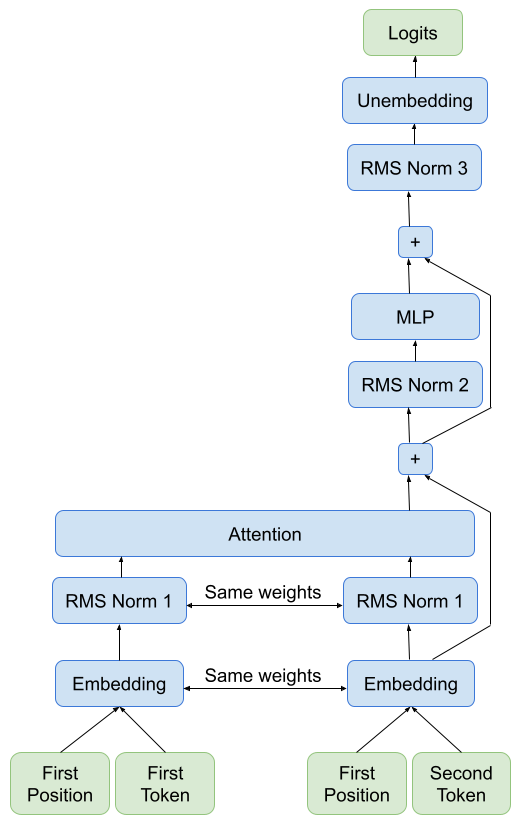
\includegraphics[width=0.5\textwidth]{Memory Toy Model - Full.png} 
\end{center}
\caption{The full toy transformer model, with all the diffrent parts pressent.}
\label{fig:full}
\end{figure}

\subsection{Model variations}

\subsubsection{Attention}
There are the variants when it comes to the attention.

\begin{itemize}
    \item \textbf{None:}
    There is no attention head, and no possitional embedding. Instead there is two diffrent token embeddings, one for each possition. These are simply added toghether to make the first recidual stream activation.

    \item \textbf{Uniform:}
    We remove the attention pathern $\mathrm{softmax}(QK^\top)$ and relace it with a uniform $\frac{1}{2}$.

    \item \textbf{Full:}
    Just norma attention.

\end{itemize}

\subsection{MLP}
There are a number of variants regarnding the MLP. Firstly the MLP can either be pressent or be missing. Secondly if there is an MLP layer, each of the follwing can be varried
\begin{itemize}
    \item \textbf{Activation Function} can be either $\mathrm{GELU}$ or $\mathrm{ReLU}$
    \item \textbf{Bias} can exist or not.\footnote{If the bias is pressent that means both the linear readout and the linaer projection from the ReLU or GELU neurons, have bias. (Making them actualy not linear functions but affine fucntion, in strict math therminology.) If there is no bias, this means nether of these have bias. All other linear connections in the rest of the network (e.g. embeddings, etc) are alwatys bias free.}
    \item \textbf{Recidual connection} around the MLP can exist or not.
\end{itemize}

\subsection{Norms}
The norms can also be turned on and off. Each of the norms for the readin to the attention and MLP only exist if both that part of the network is pressent (Uniform or Full for the attention), and Norms are turned on. The last norm, just before the unembedding only depends on the norm setting, and are there if norms are turned on and not there if norms are turned off.

\section{First experiment and result: What parts of the network matters?}

We trained all diffrent versions of the toy model, to see how many facts each of them could learn. There are some patherns, but unfortunatly for most of them, we can't sepperate what is due to expresability of the model and what is due to leanability.

We say that a model has "learned a fact" if: When the model is given the first two tokens of this sequence, it correctly predicts the correct fird token. And by "correctly predics" we mean that argmaxing over the logits locates the correct ouput token.

To find out the maximum number of facts a model can learn, we performed a binary search over number of facts, to find the highest number of facts such that the model leaned all of them.

For each number of facts we trained 11 models in paralell, with the exact same facts, but diffrent random initialised weights. We used three diffrent success criterions "Any", "Most" and "All", meaning that we said the the model succeeded at learning all the facts, if it succedeed in any, most or all of the the 11 trials. 

We then ran each of these experiments 4 times, to check for stability. The "Any" setting had highest stabiltity (similar max numer of fact over all 4 duplicate experiments), and "All" had the worst stability.\footnote{It's not supprising that "All" had bad stability, since it only takes one bad run to though off the entire bathc. But it was not apriory obvious to us that "Any" would be more stable than "Most".}

All the results for all the experiemnst are shown in table \ref{tab:e5}.

\subsection{Norms + No Recidual around MLP + No Bias + ReLU = Bad}
This combination is bad for some reason. We don't know why. 

\subsection{No Attention > Uniform Attention > Full Attention}
It's not supprising that no attention does the best, since the dual embedding that we use to replace attention is (arguably) more powerfull. Becasuse attention is non-linear, and the dual embedding is linear, there are thing that the attention can express that the dual embdding can't. But on the other hand, the dual embedding get's to encode the input for each token possition entirely seperatly, which gives the netowrk more freedom. Addtionaly, the no attention setup should be easier to train, since it's simpler.

More supprising is that uniform attention is out performing full attenion, given that full attention is strictly more powerfull. Therefore this has to be becasue of ease of training. This interpetation is also suppored by the fact that the number of fact these netorks can learn is very varaible. We can see this in that in the number of outliers in table \ref{table:e5} and also how much number of facts dropp from Any to Majority to All.


\subsection{MLP}
Removing the MLP approximaly cutts the numner of leanable facts in half. 

\subsection{Norms}
Norms are generaly usfull for learning more facts, with one exception. If the recidual stream around the MLP is turned off, and the MLP bias is turned of, and the activation function is GELU, then and only then, does the norm make the network performe worse. This is true for all trhee settings of the attention.

If ther is no MLP the norm inceases the number of leanable facts with 79\% - 191.7\%\footnote{Based on data from "Any" the numbers are similar for "Majority" and larger for "All"}

In the rest of the settings, having norms is increasing the number of learnable facts with 2.2\% - 42.2\%\footnote{Same as last footnote}

\subsection{Recidual Connection around the MLP}
Adding this recidual connection increases the number of leanable facts with 3.1\% - 34\% \footnote{Based on data from "Any" the numbers are typially larger for "Majority" and larger for "All"}

The one outlier is the case Norm + No Bias + GeLU, where adding a Norm makes a much larger diffrence, becasue of the extra bad synergy of Norms + No Recidual around MLP + No Bias

\subsection{Activation Function}
GELU is typically better than ReLU. The diffrence is typically small -0.2\% to +12.7\% from chaning from ReLU to GELU.

Again the exception is Norm + No Recidual around the MLP + No Bias, where swiching from ReLU to GELU boosts the number of leanable facts with 58\% - 79\%.

\begin{figure}[h]
    \begin{center}
            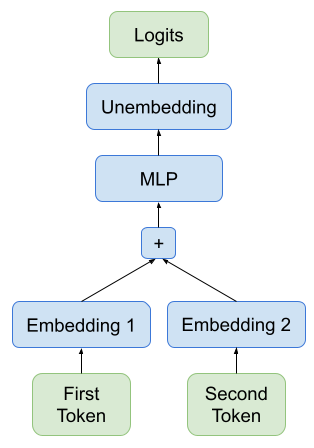
\includegraphics[width=0.5\textwidth]{Memory Toy Model - Simple.png}
    \end{center}
    \caption{A simplified version of the toy model. The MLP is pressent but everything else (attention, nomrs, recidual connection around the MLP) is turned off.}
    \label{fig:simple}
\end{figure}



\begin{table}[h]
\footnotesize
\setlength{\tabcolsep}{4.5pt}
\renewcommand{\arraystretch}{0.82}
\setlength{\fboxsep}{1.5pt}  % tighter outlier boxes (\fbox) so they don't widen the table
% Table is wider than the text block; bleed into the margins (more on the left).
\begin{adjustwidth}{-2cm}{-1.2cm}
\centering
\begin{tabular}{@{}cccccc|cccc|cccc|cccc@{}}
\toprule
 &  &  &  &  &  & \multicolumn{4}{|c}{\textbf{Any of 11}} & \multicolumn{4}{|c}{\textbf{Most of 11}} & \multicolumn{4}{|c}{\textbf{All of 11}} \\
\cmidrule(lr){7-10}\cmidrule(lr){11-14}\cmidrule(lr){15-18}
\textbf{Attn} & \textbf{MLP} & \textbf{Norm} & \textbf{Res} & \textbf{Bias} & \textbf{Act} & (1) & (2) & (3) & (4) & (1) & (2) & (3) & (4) & (1) & (2) & (3) & (4) \\
\midrule
None & \cmark & \xmark & \xmark & \xmark & GELU & 776 & 760 & 784 & \textbf{896} & 688 & 672 & \textbf{704} & \textbf{704} & \textbf{640} & 560 & 600 & 560 \\
None & \cmark & \xmark & \xmark & \xmark & ReLU & 664 & 688 & 736 & \textbf{816} & 568 & 568 & 504 & \textbf{576} & 416 & \fbox{184} & \fbox{\textbf{448}} & 288 \\
None & \cmark & \xmark & \xmark & \cmark & GELU & 864 & 848 & 896 & \textbf{904} & 776 & \textbf{800} & 784 & 792 & 680 & 680 & 680 & \textbf{720} \\
None & \cmark & \xmark & \xmark & \cmark & ReLU & \textbf{960} & 824 & 872 & 872 & 680 & \textbf{720} & 688 & 712 & 488 & 472 & \textbf{528} & 496 \\
\hdashline[1pt/3pt]
None & \cmark & \xmark & \cmark & \xmark & GELU & 992 & 984 & 984 & \textbf{1008} & 952 & \textbf{960} & 952 & \textbf{960} & 920 & \textbf{928} & 912 & \textbf{928} \\
None & \cmark & \xmark & \cmark & \xmark & ReLU & \textbf{976} & 960 & 968 & \textbf{976} & 928 & 920 & 920 & \textbf{936} & \textbf{912} & 888 & \textbf{912} & 896 \\
None & \cmark & \xmark & \cmark & \cmark & GELU & 1000 & \textbf{1008} & 992 & \textbf{1008} & 952 & \textbf{968} & 960 & 960 & \textbf{920} & \textbf{920} & \textbf{920} & \textbf{920} \\
None & \cmark & \xmark & \cmark & \cmark & ReLU & 984 & 976 & \textbf{1000} & 976 & 936 & 928 & \textbf{944} & 920 & 904 & 904 & \textbf{928} & 912 \\
\hdashline[1pt/3pt]
None & \cmark & \cmark & \xmark & \xmark & GELU & 888 & 888 & 920 & \textbf{960} & 824 & \textbf{856} & 832 & 824 & 792 & 792 & 776 & \textbf{800} \\
None & \cmark & \cmark & \xmark & \xmark & ReLU & 472 & 560 & 552 & \textbf{576} & 328 & 328 & \fbox{248} & \textbf{344} & \fbox{\textbf{256}} & 168 & \fbox{88} & 168 \\
None & \cmark & \cmark & \xmark & \cmark & GELU & \textbf{1024} & \textbf{1024} & \textbf{1024} & \textbf{1024} & \textbf{1024} & \textbf{1024} & \textbf{1024} & \textbf{1024} & 984 & 952 & \textbf{1000} & 984 \\
None & \cmark & \cmark & \xmark & \cmark & ReLU & \textbf{1024} & \textbf{1024} & \textbf{1024} & \textbf{1024} & 880 & 888 & \textbf{976} & 920 & 528 & 480 & \textbf{536} & \textbf{536} \\
\hdashline[1pt/3pt]
None & \cmark & \cmark & \cmark & \xmark & GELU & \textbf{1024} & \textbf{1024} & \textbf{1024} & \textbf{1024} & 1000 & 1016 & \textbf{1024} & \textbf{1024} & 984 & \textbf{992} & 984 & 952 \\
None & \cmark & \cmark & \cmark & \xmark & ReLU & \textbf{1024} & \textbf{1024} & \textbf{1024} & \textbf{1024} & 1016 & \textbf{1024} & \textbf{1024} & \textbf{1024} & \textbf{1008} & 984 & 992 & 992 \\
None & \cmark & \cmark & \cmark & \cmark & GELU & \textbf{1024} & \textbf{1024} & \textbf{1024} & \textbf{1024} & \textbf{1024} & \textbf{1024} & \textbf{1024} & \textbf{1024} & \textbf{1024} & \textbf{1024} & 1000 & \textbf{1024} \\
None & \cmark & \cmark & \cmark & \cmark & ReLU & \textbf{1024} & \textbf{1024} & \textbf{1024} & \textbf{1024} & \textbf{1024} & \textbf{1024} & \textbf{1024} & \textbf{1024} & 1008 & \textbf{1024} & \textbf{1024} & 1008 \\
\hdashline[1pt/3pt]
None & \xmark & \xmark & N/A & N/A & N/A & \textbf{208} & \textbf{208} & \textbf{208} & \textbf{208} & \textbf{208} & \textbf{208} & \textbf{208} & \textbf{208} & \textbf{208} & \textbf{208} & \textbf{208} & \textbf{208} \\
None & \xmark & \cmark & N/A & N/A & N/A & \textbf{576} & \textbf{576} & \textbf{576} & 552 & 536 & \textbf{544} & 528 & \textbf{544} & 496 & 480 & 472 & \textbf{504} \\
\midrule
Unif & \cmark & \xmark & \xmark & \xmark & GELU & \textbf{696} & 680 & 680 & 688 & \textbf{576} & 536 & 552 & 552 & 440 & 424 & \textbf{480} & 464 \\
Unif & \cmark & \xmark & \xmark & \xmark & ReLU & 640 & 640 & 616 & \textbf{672} & 472 & \textbf{512} & 480 & \textbf{512} & 336 & 376 & 368 & \textbf{392} \\
Unif & \cmark & \xmark & \xmark & \cmark & GELU & 712 & 696 & \textbf{720} & \textbf{720} & 664 & 640 & 632 & \textbf{672} & \textbf{528} & 520 & 488 & 520 \\
Unif & \cmark & \xmark & \xmark & \cmark & ReLU & 712 & 712 & 704 & \textbf{720} & \textbf{640} & \textbf{640} & 584 & \textbf{640} & 448 & 440 & \textbf{480} & 432 \\
\hdashline[1pt/3pt]
Unif & \cmark & \xmark & \cmark & \xmark & GELU & \textbf{832} & 824 & 824 & 816 & 792 & 792 & \textbf{800} & 792 & \textbf{768} & 720 & 744 & 760 \\
Unif & \cmark & \xmark & \cmark & \xmark & ReLU & \textbf{816} & 808 & \textbf{816} & 800 & 760 & 776 & \textbf{784} & \textbf{784} & 736 & \textbf{744} & 728 & \fbox{504} \\
Unif & \cmark & \xmark & \cmark & \cmark & GELU & 824 & 832 & \textbf{840} & \textbf{840} & 800 & \textbf{808} & 800 & \textbf{808} & 728 & 760 & \textbf{776} & 752 \\
Unif & \cmark & \xmark & \cmark & \cmark & ReLU & \textbf{824} & 792 & 816 & 800 & \textbf{784} & 776 & \textbf{784} & \textbf{784} & 760 & \textbf{768} & \textbf{768} & 760 \\
\hdashline[1pt/3pt]
Unif & \cmark & \cmark & \xmark & \xmark & GELU & \textbf{800} & \textbf{800} & 776 & 784 & \textbf{744} & 736 & \textbf{744} & 736 & 696 & 696 & 696 & \textbf{704} \\
Unif & \cmark & \cmark & \xmark & \xmark & ReLU & 496 & 504 & \textbf{528} & 440 & 280 & 296 & \textbf{312} & 248 & 104 & 144 & 104 & \fbox{\textbf{160}} \\
Unif & \cmark & \cmark & \xmark & \cmark & GELU & 880 & \textbf{904} & 888 & 888 & \textbf{848} & \textbf{848} & \textbf{848} & 840 & \textbf{776} & 760 & \textbf{776} & 768 \\
Unif & \cmark & \cmark & \xmark & \cmark & ReLU & \textbf{920} & 888 & 896 & 880 & \textbf{768} & 728 & \textbf{768} & \textbf{768} & 240 & 248 & 248 & \fbox{\textbf{448}} \\
\hdashline[1pt/3pt]
Unif & \cmark & \cmark & \cmark & \xmark & GELU & 880 & 896 & 912 & \textbf{920} & 856 & \textbf{864} & 848 & 856 & \textbf{832} & 816 & 800 & 792 \\
Unif & \cmark & \cmark & \cmark & \xmark & ReLU & 872 & 880 & \textbf{904} & 872 & \textbf{856} & 840 & 848 & \textbf{856} & 800 & 792 & 800 & \textbf{808} \\
Unif & \cmark & \cmark & \cmark & \cmark & GELU & 944 & 936 & \textbf{960} & \textbf{960} & \textbf{912} & 904 & 904 & 896 & 856 & 864 & \textbf{880} & 856 \\
Unif & \cmark & \cmark & \cmark & \cmark & ReLU & 912 & 944 & 936 & \textbf{960} & \textbf{896} & 888 & 888 & 872 & 816 & \textbf{832} & \textbf{832} & \textbf{832} \\
\hdashline[1pt/3pt]
Unif & \xmark & \xmark & N/A & N/A & N/A & \textbf{208} & \textbf{208} & \textbf{208} & \textbf{208} & 200 & 192 & \textbf{208} & 192 & \textbf{192} & \textbf{192} & \textbf{192} & \textbf{192} \\
Unif & \xmark & \cmark & N/A & N/A & N/A & \textbf{416} & 408 & 408 & 408 & \textbf{376} & \textbf{376} & \textbf{376} & \textbf{376} & 312 & 304 & 328 & \textbf{336} \\
\midrule
Full & \cmark & \xmark & \xmark & \xmark & GELU & 536 & 584 & 504 & \textbf{600} & \fbox{304} & \textbf{392} & 384 & 384 & \fbox{\textbf{136}} & 120 & \fbox{80} & 88 \\
Full & \cmark & \xmark & \xmark & \xmark & ReLU & 456 & 576 & 488 & \textbf{584} & 312 & \textbf{352} & 272 & 312 & \fbox{112} & \fbox{64} & \fbox{\textbf{128}} & \fbox{48} \\
Full & \cmark & \xmark & \xmark & \cmark & GELU & 600 & 632 & \textbf{696} & 616 & 336 & \textbf{384} & 312 & 352 & \fbox{144} & \fbox{\textbf{152}} & \fbox{24} & \fbox{48} \\
Full & \cmark & \xmark & \xmark & \cmark & ReLU & 544 & \textbf{656} & 536 & 640 & 280 & 272 & \textbf{368} & 360 & \fbox{\textbf{144}} & \fbox{16} & 72 & 56 \\
\hdashline[1pt/3pt]
Full & \cmark & \xmark & \cmark & \xmark & GELU & \textbf{688} & 664 & 656 & 640 & 344 & 328 & \textbf{384} & \fbox{248} & \fbox{56} & \fbox{128} & \fbox{\textbf{136}} & \fbox{40} \\
Full & \cmark & \xmark & \cmark & \xmark & ReLU & \fbox{488} & 672 & \textbf{704} & 688 & \textbf{336} & 320 & 248 & 248 & 88 & \fbox{\textbf{112}} & 64 & 72 \\
Full & \cmark & \xmark & \cmark & \cmark & GELU & 624 & 664 & \textbf{712} & 608 & 264 & 296 & 248 & \textbf{328} & \fbox{16} & \fbox{\textbf{128}} & \fbox{96} & \fbox{56} \\
Full & \cmark & \xmark & \cmark & \cmark & ReLU & \textbf{648} & 600 & 504 & 592 & 272 & 248 & \fbox{176} & \fbox{\textbf{512}} & 96 & \fbox{64} & 80 & \fbox{\textbf{112}} \\
\hdashline[1pt/3pt]
Full & \cmark & \cmark & \xmark & \xmark & GELU & \textbf{784} & 768 & 768 & 696 & 648 & \textbf{656} & 600 & 616 & 264 & \fbox{\textbf{368}} & 232 & 232 \\
Full & \cmark & \cmark & \xmark & \xmark & ReLU & 440 & \textbf{512} & 496 & 472 & 312 & 296 & 320 & \textbf{328} & 128 & \fbox{\textbf{192}} & 152 & 136 \\
Full & \cmark & \cmark & \xmark & \cmark & GELU & 800 & \textbf{896} & 800 & 760 & 600 & 672 & \fbox{504} & \textbf{704} & 336 & \fbox{184} & \textbf{376} & 296 \\
Full & \cmark & \cmark & \xmark & \cmark & ReLU & 800 & 776 & 728 & \textbf{832} & 440 & 520 & \textbf{576} & 536 & \fbox{152} & 232 & 264 & \textbf{288} \\
\hdashline[1pt/3pt]
Full & \cmark & \cmark & \cmark & \xmark & GELU & \textbf{864} & 776 & 832 & 808 & 632 & 704 & \textbf{736} & 704 & 232 & 216 & \fbox{\textbf{320}} & 184 \\
Full & \cmark & \cmark & \cmark & \xmark & ReLU & 776 & \textbf{832} & \textbf{832} & \textbf{832} & 680 & 688 & \textbf{728} & 688 & 280 & 240 & 280 & \textbf{296} \\
Full & \cmark & \cmark & \cmark & \cmark & GELU & 848 & 816 & \textbf{872} & 808 & \textbf{720} & 696 & 632 & 704 & 320 & \fbox{248} & 384 & \fbox{\textbf{448}} \\
Full & \cmark & \cmark & \cmark & \cmark & ReLU & 832 & \textbf{840} & \textbf{840} & 792 & \textbf{768} & 704 & 640 & 632 & \textbf{336} & \fbox{208} & 320 & 240 \\
\hdashline[1pt/3pt]
Full & \xmark & \xmark & N/A & N/A & N/A & 208 & 168 & \textbf{224} & 208 & 112 & \textbf{120} & 88 & 96 & 16 & 16 & 16 & \fbox{\textbf{48}} \\
Full & \xmark & \cmark & N/A & N/A & N/A & 384 & \fbox{272} & \textbf{416} & 384 & 168 & 176 & \fbox{136} & \textbf{192} & \textbf{64} & 48 & 56 & 56 \\
\bottomrule
\end{tabular}

\end{adjustwidth}
\caption{Maximum facts memorised per architectural configuration ($d_\text{residual}=16$, $d_\text{ff}=16$, CE loss). \textbf{Attn} is the token-mixing mechanism: \emph{None} (additive per-position embeddings), \emph{Unif} (uniform/averaging attention, \texttt{qk\_is\_one = True}), or \emph{Full} (learned attention). The \emph{Any} / \emph{Majority} / \emph{All} column groups apply the corresponding criterion (a fact count counts as learned if at least one / more than half / all of the $11$ attempts reach perfect accuracy); the four numbered columns within each group are independent repeats. Within each group the row-wise maximum is shown in \textbf{bold} and values more than $20\%$ from the group's median are \fbox{boxed} as outliers. For \texttt{ff = False} rows the residual, bias and activation flags do not apply (N/A). Note that $1024$ is the dataset ceiling, so configurations reaching it have saturated the data rather than the model.}
\label{tab:e5}
\end{table}


\section{Challange / Benchmark for understanding}
Can you or me, write down weights for the memory toy model, eitgher by hand or some algorithm that isn't gradient decent, such that our resulting model match the performance of the leaned model?

This chalance is benchmark for how well we understand how the model store the facts. There are two reasons why this is a usefull frameing.
\begin{itemize}
    \item If we understand how the facts are embedded, we should be able to replicate this, whithout gadient decaent.
    \item Fhinkging about "How would I do this?" can be a usefull framing for mech-interp.
\end{itemize}

We think that our current best attempt (which will be pressented soon) is some non-zero progress on this challange, but there are still far to go. We encurrage all readers go give it a try.

\subsection{Model architecture}
Firstly, we're not trying (yet) to produce weights for the full tranformer model, but instead aiming to find functional weights for the simplified toy model shown in figure \ref{fig:simple}

Seconldy, the version shown in \ref{fig:simple} has unessearely many weights, wich is a legacy from being a cutt down version of the full version shown in \ref{fig:full}. Because the MLP is sandwich between two linear operations, we can skipp the weight matrices of the MLP.

We can simplify it further down to this: See figure \ref{fig:hc}

\begin{figure}[h]
    \begin{center}
            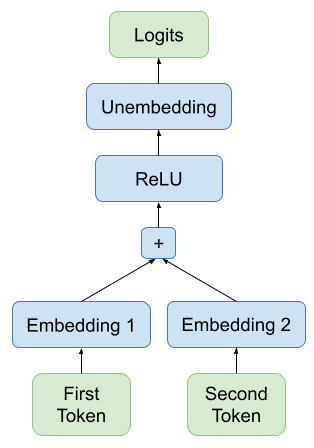
\includegraphics[width=0.5\textwidth]{Memory Toy Model - Hand Coded.png}
    \end{center}
    \caption{This model is equivalent to the toy model configuration with settings Attn=None, FF=ON, Norm=OFF, Res=OFF, Bias=OFF, Act=ReLU.}
    \label{fig:hc}
\end{figure}

If you want to give the challage a go, feel free to use this architecture, of any other that you find easier to work with. The final goal is to be able to write down functional weights for the full transformer model, but we think it's ok to start with a simpler case. 

\subsection{Our attempt}
Our algorithm has three steps
\begin{itemize}
    \item Assign $S$ number ReLU neurons to each label. This means that each neuron will be assigned to several labels. We try to generate an assigment that accives both: Each neuron should have approximatly the same labels assigned to it as any other neuron; The max neuron overlap between any pair of labels, should be as small as possible.
    \item Chose the embeding weighs such that each ReLU neuron assigned to label $l$ will output zero for all facts with label $l$.
    \item Assigned a lage negativ weiths from ReLU neurons assigned to $l$ to the logit for $l$. Assign small possitive weights everywhere else.
\end{itemize}

\subsubsection{Assigning neurons to labels}

\subsubsection{Embedding weights}

\subsection{Unembedding weights}

\end{document}